\documentclass[12pt]{article}
\usepackage{amsmath, amssymb}
\usepackage{hyperref}
\usepackage{fancyhdr} % 添加页眉页脚功能
\usepackage{graphicx} % 用于插入图片
\usepackage{float} % 用于控制图片位置

\setlength{\parindent}{0pt}
\setlength{\parskip}{1em}

% 设置页眉和页脚样式
\pagestyle{fancy}
\fancyhf{} % 清空当前的页眉页脚设置
\fancyhead[L]{Assignment 1 NIE, Weihao (SID: 20945074)} % 左侧页眉
\fancyhead[R]{COMP 5214 (2025 Spring)} % 右侧页眉
\renewcommand{\headrulewidth}{0.4pt} % 页眉下的横线宽度

\begin{document}

\begin{center}
    {\Large \textbf{Assignment 1 Report}}
    
    NIE, Weihao \\
    COMP 5214 (2025 Spring) \\
    
    \vspace{1em}
    \begin{tabular}{ll}
        \textbf{Name:} NIE, Weihao & \textbf{Student ID:} 20945074 \\
    \end{tabular}
\end{center}

\section{Introduction}
In this assignment, we implements four models to solve the classification problem on MNSIT dataset. 
The four models are: \textbf{MLP, KNN, CNN} and \textbf{CAN}. We will train the models on the training set and evaluate the models on the test set.
The performance of each models will be compared and analyzed in the following sections.
The answer of questions mentioned in the assignment decription will also be provided in the corresponding sections.

\section{Models}

\subsection{KNN}

In this part, I implement the KNN model to solve the classification problem on MNSIT dataset.
The KNN model is implemented by using the \texttt{KNeighborsClassifier} class in the \texttt{sklearn} library.
The performance of the KNN model versus the number of neighbors is shown in Figure \ref{fig:knn_accuracy}.

\begin{figure}[H] % 使用 [H] 参数确保图片在当前位置
  \centering
  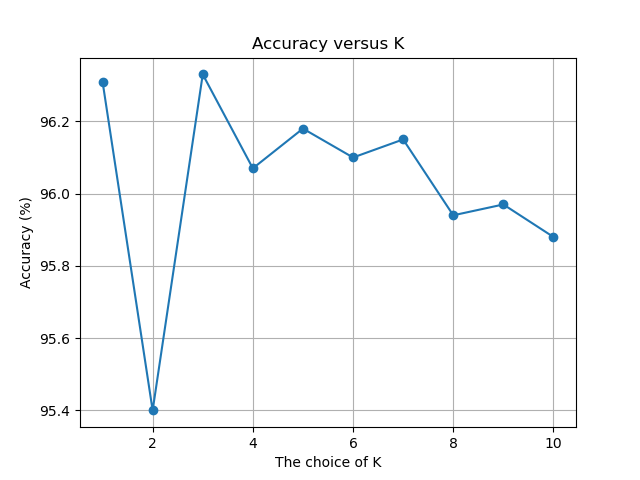
\includegraphics[width=0.8\textwidth]{KNN.png} % 确保路径正确
  \caption{KNN Accuracy vs K Values.}
  \label{fig:knn_accuracy} % 设置引用标签
\end{figure}

From the figure, we can see that when we choose the nearest neighbor, the accuracy is the second highest.
The highest accuracy is achieved when we choose 3 neighbors.
However, when the number of neighbors is 2, the accuracy is the lowest.
This is may because when we choose 2 neighbors, the model is overfitting on the training set.

\subsection{MLP}

In this part, I implement the MLP model to solve the classification problem on MNSIT dataset.
The MLP consists of 2 hidden layers with same number of neurons.
In this model, I use Relu as the activation function and SGD as the optimizer.
The performance of the MLP model versus the number of neurons is shown in Figure \ref{fig:mlp_accuracy}.

\begin{figure}[H] % 使用 [H] 参数确保图片在当前位置
  \centering
  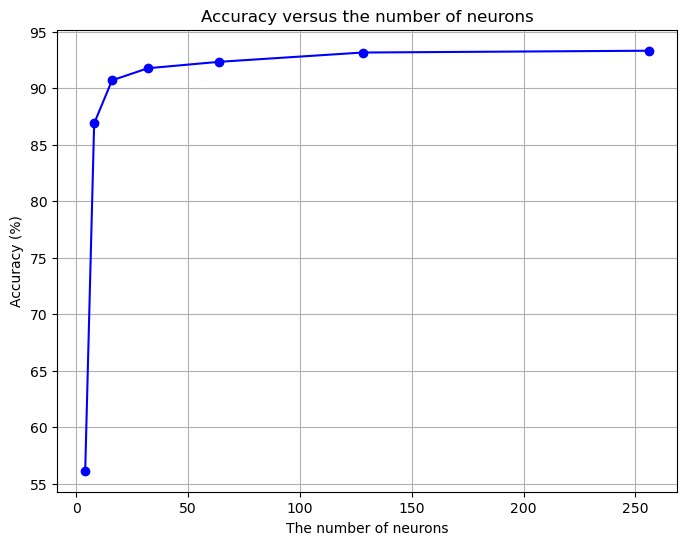
\includegraphics[width=0.8\textwidth]{MLP.png} % 确保路径正确
  \caption{MLP Accuracy vs number of neurons.}
  \label{fig:mlp_accuracy} % 设置引用标签
\end{figure}

From the figure, we can see that when we choose 256 neurons, the accuracy is the highest.
When we choose 128 neurons, the accuracy is the second highest.
The performance of the model improves as the number of neurons increases.
This is may because the model can learn more complex patterns with more neurons.

\subsection{CNN}

In this part, I implement the CNN model following the LeNet-5 architecture.
After training the model, the accuracy on the test set is 98.63\text{\%}.
The performance of the CNN model is much better than the MLP, which means that the CNN model can learn more complex patterns than the MLP model.

\subsection{CAN}

In this part, I implement the CAN model following the architecture in the assignment description.
The performance of the CAN model versus the number of channels is shown in Figure \ref{fig:can_accuracy}.

\begin{figure}[H]
  \centering
  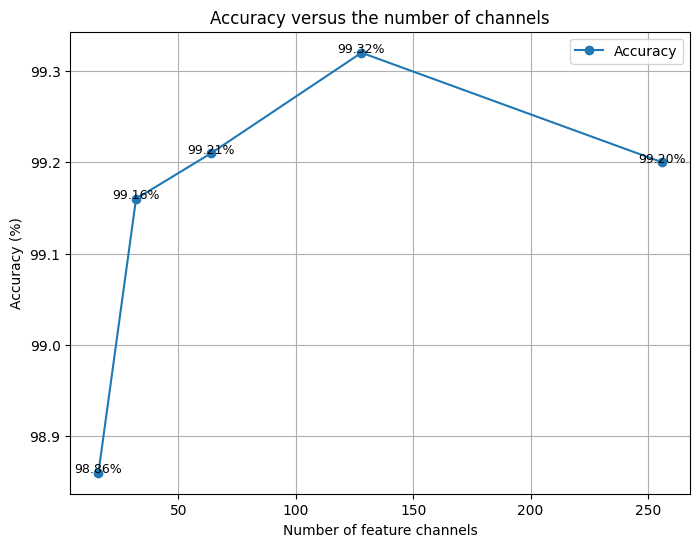
\includegraphics[width=0.8\textwidth]{CAN.png}
  \caption{CAN Accuracy vs number of channels.}
  \label{fig:can_accuracy}
\end{figure}

From the figure, we can see that when we choose 128 channels, the accuracy is the highest.
When we choose 16 channels, the accuracy is the second lowest.
I notice that when the number of channels is under 128, the accuracy improves with the increasement of channels number.
However, when the number of channels is over 128, the accuracy decreases with the increasement of channels number.
This is may because the model is overfitting on the training set when the number of channels is too large.

\end{document}